\documentclass[10pt, aspectratio=149]{beamer}

% Include preamble files
% Package imports
\usepackage{media9}
\usepackage{amssymb,amsmath,amsthm,enumerate}
\usepackage[utf8]{inputenc}
\usepackage{array}
\usepackage[parfill]{parskip}
\usepackage{graphicx}
\usepackage{caption}
\usepackage{subcaption}
\usepackage{bm}
\usepackage{amsfonts,amscd}
\usepackage[]{units}
\usepackage{listings}
\usepackage{multicol}
\usepackage{multirow}
\usepackage{tcolorbox}
\usepackage{physics}
\usepackage{algorithm2e}
\usepackage{lastpage}
\usepackage{pifont}
\usepackage{animate}
\usepackage{ifthen}
\usepackage{hyperref}
\usepackage{pgffor}
\usepackage[margin=1in]{geometry}
\usepackage[acronym]{glossaries}
\usepackage[style=ieee]{biblatex}
% \lstset{basicstyle=\ttfamily\small} % optional settings

\lstset{
  basicstyle=\ttfamily\small,
  keywordstyle=\color{blue},
  commentstyle=\color{gray},
  breaklines=true
}

% Enable colored hyperlinks
\hypersetup{colorlinks=true}

% Numbered captions of tables, pictures, etc.
\setbeamertemplate{caption}[numbered]

% Bibliography settings
\setbeamertemplate{bibliography item}{\insertbiblabel}
\addbibresource{references.bib} 

% --- Customization for enumerated ToC ---
% Set templates for sections and subsections in the ToC to be numbered
% Even vertical spacing and top alignment for ToC items, with top/bottom padding
\setbeamertemplate{section in toc}[sections numbered]
\setbeamertemplate{toc item}{\vspace{0.7em}} % Adjust spacing as needed
\addtobeamertemplate{frametitle}{}{\vspace*{-\baselineskip}} % Remove extra space above ToC
\setbeamertemplate{toc}{%
  \vbox{%
    \vspace*{1.5em} % Top padding
    \insertbeamertoc
    \vspace*{1.5em} % Bottom padding
  }
}
% Indent subsections in ToC by 4 spaces and put each on a new line
\setbeamertemplate{subsection in toc}{%
  \par\hspace*{1em}\inserttocsubsectionnumber.\;\inserttocsubsection%
}
% --- End Customization ---

% Custom commands
\newcommand{\R}{\mathbb{R}}
\renewcommand{\thealgocf}{}

% Crossmarks & checkmarks
\newcommand{\cmark}{\ding{51}}
\newcommand{\xmark}{\ding{55}}

% Colored emphasis
\newcommand{\empy}[1]{{\color{darkorange}\emph{#1}}}
\newcommand{\empr}[1]{{\color{blue}\emph{#1}}}

% A command to fetch an image via curl if it doesn't yet exist
\newcommand{\fetchimage}[2]{%
  \IfFileExists{#1}{}{%
    \immediate\write18{curl -sL "#2" -o "#1"}%
  }%
}

% Robust macro to fetch and convert web image to PNG for LaTeX
% Requires shell-escape, curl, and ImageMagick (convert)
\newcommand{\fetchconvertimageonly}[2]{%
  \IfFileExists{#2}{}{%
    \immediate\write18{curl -sL "#1" -o "temp_image_download"}%
    \immediate\write18{convert temp_image_download "#2"}%
    \immediate\write18{rm -f temp_image_download}%
  }%
}

% Robust macro to fetch and convert web image to PNG for LaTeX
% Requires shell-escape, curl, and ImageMagick (convert)
\newcommand{\fetchconvertimage}[3]{%
  \IfFileExists{#2}{}{%
    \immediate\write18{curl -sL "#1" -o "temp_image_download"}%
    \immediate\write18{convert temp_image_download "#2"}%
    \immediate\write18{rm -f temp_image_download}%
  }%
  \includegraphics[#3]{#2}%
}

% Adaptive macro to convert a GIF into frames and animate it
% Usage: \includeGIF{your.gif}{basename}{width}{fps}
\newcommand{\includeGIF}[4]{%
  % % Frame path prefix
  % \def\gifpath{gif_frames}%
  % \def\frameprefix{\gifpath/#2_}%

  % % If frames don't exist, extract them
  % \IfFileExists{\frameprefix000.png}{}{%
  %   \immediate\write18{mkdir -p \gifpath}%
  %   \immediate\write18{convert "#1" "\frameprefix%03d.png"}%
  %   % Count frames using identify
  %   \immediate\write18{identify -format \%n "#1" > \gifpath/#2_framecount.txt}%
  % }%

  % % Read frame count
  % \newread\framecountfile%
  % \openin\framecountfile=\gifpath/#2_framecount.txt%
  % \read\framecountfile to \totalframes%
  % \closein\framecountfile%

  % % Decrement for zero-based indexing (e.g., 10 frames = 000 to 009)
  % \newcount\lastframe
  % \lastframe=\totalframes
  % \advance\lastframe by -1

  % % Pad last frame (e.g., 9 becomes 009)
  % \edef\lastframepad{\ifnum\lastframe<10 00\the\lastframe\else\ifnum\lastframe<100 0\the\lastframe\else\the\lastframe\fi\fi}%

  % % Animate using detected frame range
  % \animategraphics[loop,controls,width=#3]{#4}{\frameprefix}{000}{\lastframepad}%

  \begingroup
  \def\giffile{#1}%
  \def\basename{#2}%
  \def\widthval{#3}%
  \def\fpsval{#4}%
  \def\gifpath{gif_frames}%
  \def\frameprefix{\gifpath/\basename\_}%

  \IfFileExists{\frameprefix000.png}{}{%
    \immediate\write18{mkdir -p \gifpath}%
    \immediate\write18{convert "\giffile" "\frameprefix%03d.png"}%
    \immediate\write18{identify -format %%n "\giffile" > "\gifpath/\basename\_framecount.txt"}%
  }%

  \newread\framecountfile%
  \openin\framecountfile=\gifpath/\basename\_framecount.txt%
  \read\framecountfile to \totalframes%
  \closein\framecountfile%

  \newcount\lastframe
  \lastframe=\totalframes
  \advance\lastframe by -1

  % Format last frame number as zero-padded (e.g., 9 -> 009)
  \def\lastframepad{\ifnum\lastframe<10 00\the\lastframe\else%
    \ifnum\lastframe<100 0\the\lastframe\else%
    \the\lastframe\fi\fi}%

  \animategraphics[loop,controls,width=\widthval]{\fpsval}{\frameprefix}{000}{\lastframepad}%
  \endgroup
}


% Example box
\newcommand{\examplebox}[2]{
\begin{tcolorbox}[colframe=darkcardinal,colback=boxgray,title=#1]
#2
\end{tcolorbox}}

% Theorem environments
\theoremstyle{remark}
\newtheorem*{remark}{Remark}
\theoremstyle{definition}

% Glossary entries
\newacronym{ML}{ML}{machine learning} 
% Beamer settings
\usetheme{Stanford} 
\def \i  {\item}
\def \ai {\item[] \quad \arrowbullet}
\newcommand \si[1]{\item[] \quad \bulletcolor{#1}}
\def \wi {\item[] \quad $\ \phantom{\Rightarrow}\ $}
\def \bi {\begin{itemize}\item}
\def \ei {\end{itemize}}
\def \be {\begin{equation*}}
\def \ee {\end{equation*}}
\def \bie {$\displaystyle{}
\def \eie {{\ }$}}
\def \bsie {\small$\displaystyle{}
\def \esie {{\ }$}\normalsize\selectfont}
\def \bse {\small\begin{equation*}}
\def \ese {\end{equation*}\normalsize}
\def \bfe {\footnotesize\begin{equation*}}
\def \efe {\end{equation*}\normalsize}
\renewcommand \le[1] {\\ \medskip \lefteqn{\hspace{1cm}#1} \medskip}
\def \bex {\begin{example}}
\def \eex {\end{example}}
\def \bfig {\begin{figure}}
\def \efig {\end{figure}}
\def \btheo {\begin{theorem}}
\def \etheo {\end{theorem}}
\def \bc {\begin{columns}}
\def \ec {\end{columns}}
\def \btab {\begin{tabbing}}
\def \etab {\end{tabbing}\svneg\svneg}
\newcommand \col[1]{\column{#1\linewidth}}
\def\vneg  {\vspace{-5mm}}
\def\lvneg {\vspace{-10mm}}
\def\svneg {\vspace{-2mm}}
\def\tvneg {\vspace{-1mm}}
\def\vpos  {\vspace{5mm}}
\def\lvpos {\vspace{10mm}}
\def\svpos {\vspace{2mm}}
\def\tvpos {\vspace{1mm}}
\def\hneg  {\hspace{-5mm}}
\def\lhneg {\hspace{-10mm}}
\def\shneg {\hspace{-2mm}}
\def\thneg {\hspace{-1mm}}
\def\hpos  {\hspace{5mm}}
\def\lhpos {\hspace{10mm}}
\def\shpos {\hspace{2mm}}

\logo{
\includegraphics[height=0.4in]{style_files/kaust_academy_logo.png}}

% Commands to relax beamer and subfig conflicts
\makeatletter
\let\@@magyar@captionfix\relax
\makeatother

% Set itemize styles
\setbeamertemplate{itemize items}[default]
\setbeamertemplate{itemize subitem}[circle] 

\title[Normalizing Flow Models]{Normalizing Flow Models}

\begin{document}

% Include sections
% Title page
\author[LMH]{
    \begin{tabular}{c} 
    \Large
    Naeemullah Khan\\
    \footnotesize \href{mailto:naeemullah.khan@kaust.edu.sa}{naeemullah.khan@kaust.edu.sa}
    \end{tabular}
    \vspace{-4ex}
}

\institute{
    \vskip 20pt
    \begin{figure}
        \centering
        \begin{subfigure}[t]{\textwidth}
            \centering
            
\includegraphics[height=0.5in]{style_files/kaust_logo.png}
            
\includegraphics[height=0.5in]{style_files/LMHLogo.jpeg}
        \end{subfigure}
    \end{figure}
    \vskip 20pt
    % KAUST Academy \\
    % King Abdullah University of Science and Technology\\
    % \vskip 3pt 
}

\date{\today}

\begin{noheadline}
\begin{frame}\maketitle\end{frame}
\end{noheadline}
% % Title page
\author[KAUST Academy]{
    \begin{tabular}{c} 
    \Large
    Naeemullah Khan\\
    \footnotesize \href{mailto:naeemullah.khan@kaust.edu.sa}{naeemullah.khan@kaust.edu.sa}
    \end{tabular}
    \vspace{-4ex}
}

\institute{
    \vskip 20pt
    \begin{figure}
        \centering
        \begin{subfigure}[t]{0.5\textwidth}
            \centering
            
\includegraphics[height=0.5in]{style_files/kaust_logo.png}
        \end{subfigure}
    \end{figure}
    \vskip 20pt
    KAUST Academy \\
    King Abdullah University of Science and Technology\\
    \vskip 3pt
}

\date{\today}

\begin{noheadline}
\begin{frame}\maketitle\end{frame}
\end{noheadline}

% Table of Contents
\begin{frame}[allowframebreaks]{Table of Contents}
\begin{enumerate}
    \item Challenges
    \item Intersection over Union (IoU)
    \item Single Object Detection
    \item Multiple Objects & Sliding Window
    \item Region Proposal Networks (RPN)
    \item R-CNN
    \item Fast R-CNN
    \item Faster R-CNN
    \item YOLO 
    \item Summary
\end{enumerate}
\end{frame}
\section{Motivation}
\begin{frame}{Motivation}
    \large Why this topic matters:
        \begin{itemize}
            \item Traditional CNNs struggle with sequential and long-range dependencies.
            \item RNNs were a start, but they come with their own baggage.
            \item Attention mechanisms and Transformers revolutionized NLP – now transforming vision tasks.
            \item Vision Transformers (ViTs) are outperforming CNNs on many benchmarks.
            \item \textit{"Understanding the Transformer is a must for any modern deep learning practitioner."}
        \end{itemize}
\end{frame}
\begin{frame}[allowframebreaks]{\textcolor{green}{$\Rightarrow$} Learning Outcomes}
    By the end of this session, you will be able to:
    \begin{itemize}
        \item Explain what a VAE is and why we use it
        \item Describe how VAEs create and use hidden (latent) spaces
        \item Understand how VAEs learn from data
        \item Understand the ELBO and its role
        \item See how we train VAEs using special tricks
        \item Recognize different types of VAEs and some common challenges
    \end{itemize}
\end{frame}
\section{Introduction}
\begin{frame}{}
    \LARGE SSL: \textbf{Introduction}
\end{frame}

\begin{frame}[allowframebreaks]{Introduction}
    \begin{figure}
        \centering
        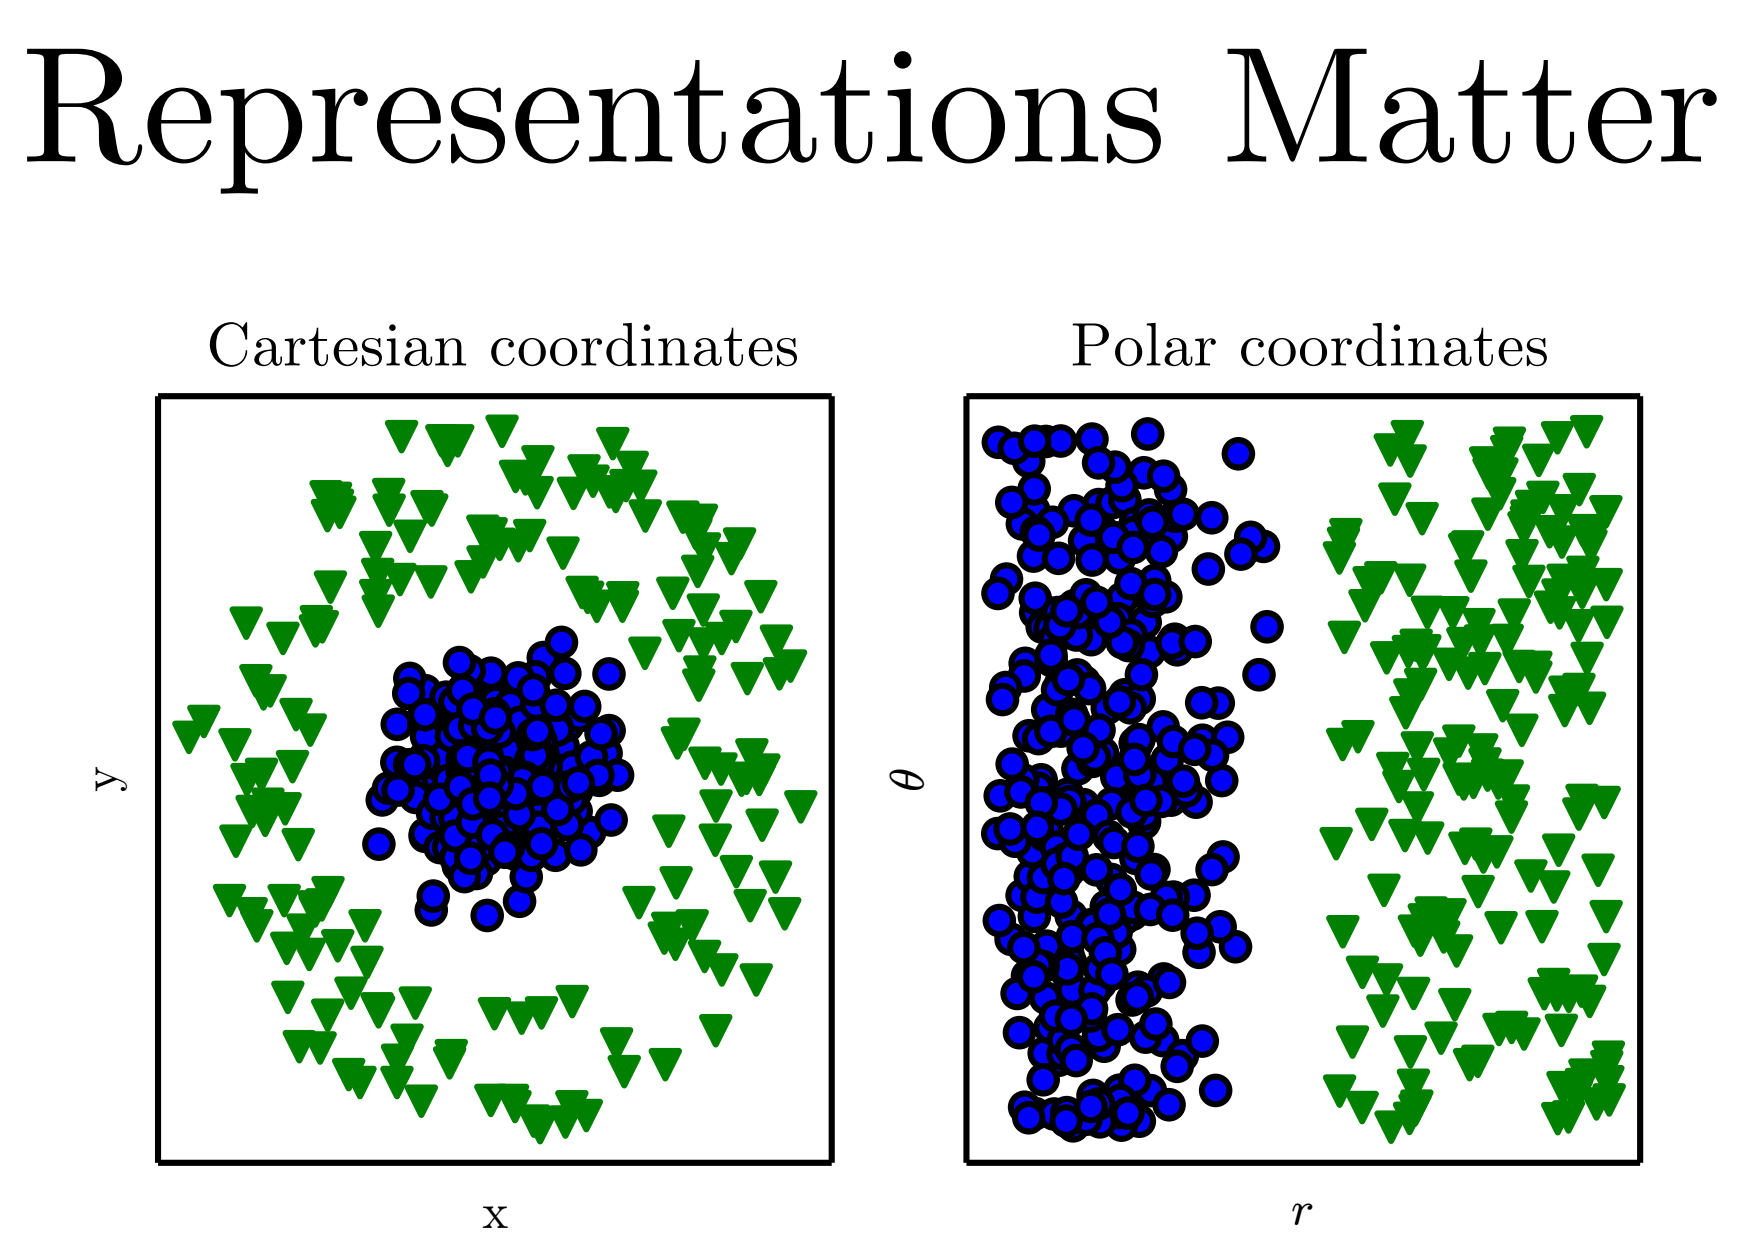
\includegraphics[width=\linewidth,height=0.9\textheight,keepaspectratio]{images/ssl/slide_2_1_img.png}
    \end{figure}

    \framebreak

    \begin{columns}
    \begin{column}{0.7\textwidth}
        \begin{figure}
            \flushleft
            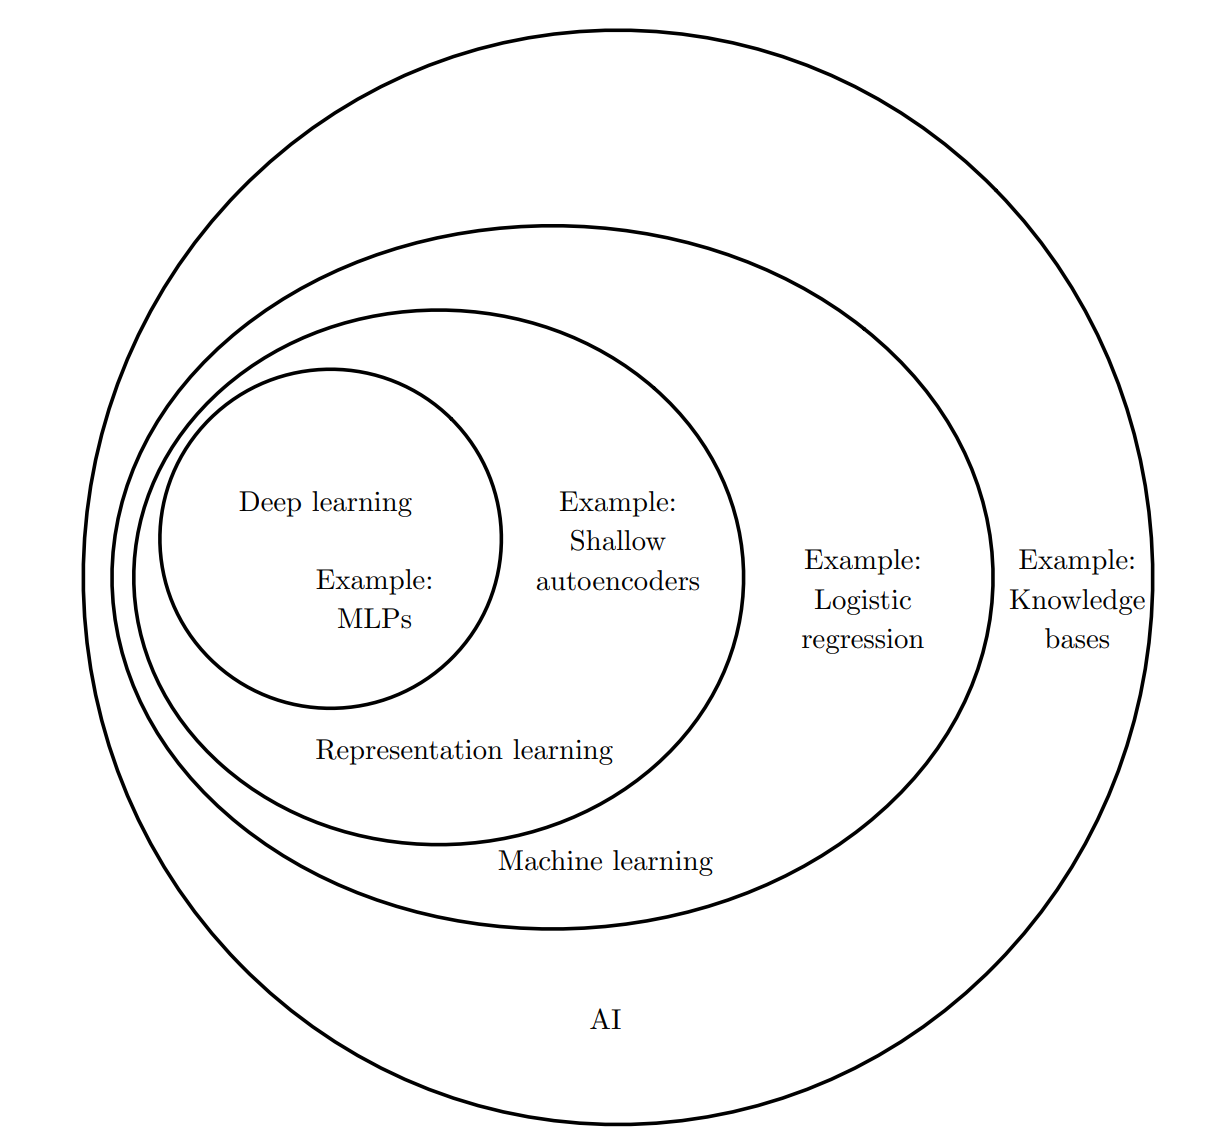
\includegraphics[width=\linewidth,height=0.8\textheight,keepaspectratio]{images/ssl/slide_3_1_img.png}
        \end{figure}
    \end{column}
    \begin{column}{0.48\textwidth}
        \textbf{Deep Unsupervised Learning:}
        \begin{itemize}
            \item Learns data representations without using labels.
            \item Is a subset of Deep Learning, which itself is a subset of Representation Learning, all within Machine Learning.
        \end{itemize}
    \end{column}
    \end{columns} 
    
    \framebreak

    \begin{columns}
    \begin{column}{0.55\textwidth}
        \begin{figure}
            \flushleft
            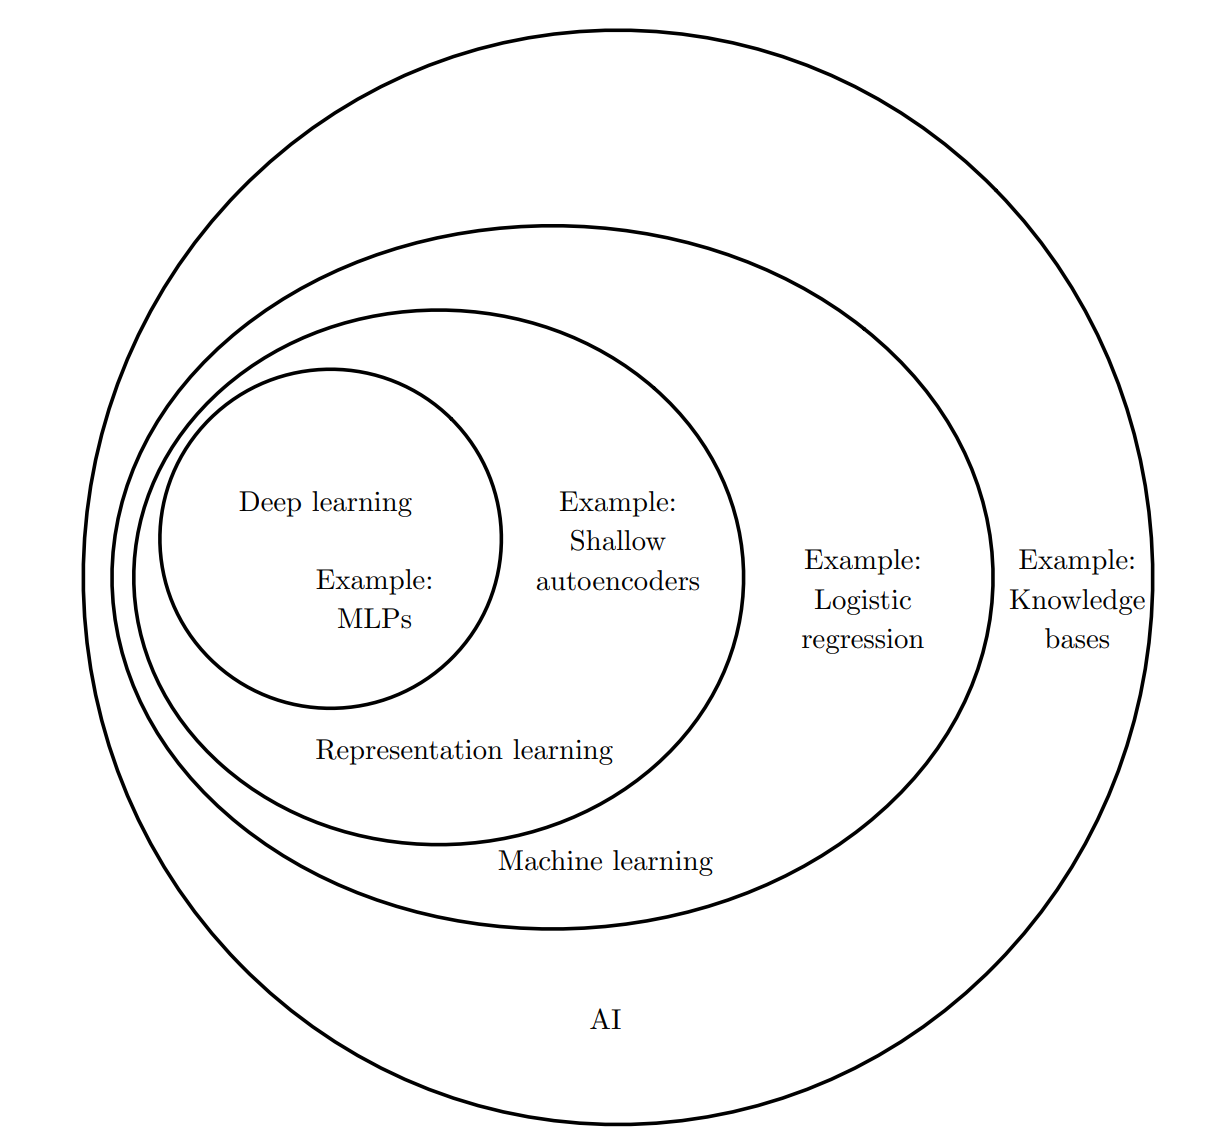
\includegraphics[width=\linewidth,height=0.8\textheight,keepaspectratio]{images/ssl/slide_3_1_img.png}
        \end{figure}
    \end{column}
    \begin{column}{0.62\textwidth}
        \textbf{Deep Unsupervised Learning:}
        \begin{itemize}
            \item Learns data representations without using labels.
            \item Is a subset of Deep Learning, which itself is a subset of Representation Learning, all within Machine Learning.
        \end{itemize}
        \vspace{0.5em}
        \textbf{Self-Supervised Learning (SSL):}
        \begin{itemize}
            \item A form of unsupervised learning that creates supervision from the data itself by designing \textit{pretext tasks}.
            \item These tasks generate pseudo-labels, enabling the model to learn useful representations without manual annotation.
            \item Often used interchangeably with unsupervised learning, but SSL specifically focuses on leveraging intrinsic data structure.
        \end{itemize}
    \end{column}
    \end{columns} 
\end{frame}

\begin{frame}[allowframebreaks]{Why Self-Supervised Learning?}
    \begin{itemize}
        \item \textbf{High cost of dataset creation:} Each new task often requires building a new labeled dataset.
        \begin{itemize}
            \item Involves preparing labeling manuals, defining categories, hiring annotators, building GUIs, and managing storage pipelines.
        \end{itemize}
        \item \textbf{Expensive supervision:} High-quality labels can be costly or impractical to obtain (e.g., in medicine or legal domains).
        \item \textbf{Leverage unlabeled data:} The internet provides vast amounts of unlabeled images, videos, and text that can be utilized.
        \item \textbf{Cognitive motivation:} Animals and babies learn from their environment without explicit supervision, inspiring SSL approaches.
    \end{itemize}

    \framebreak

    \begin{columns}
    \begin{column}{0.7\textwidth}
        \begin{figure}
            \flushleft
            
\includegraphics[width=\linewidth,height=0.8\textheight,keepaspectratio]{images/ssl/slide_7_1_img.png}
        \end{figure}
    \end{column}
    \begin{column}{0.4\textwidth}
        \textit{“Give a robot a label and you feed it for a moment; teach a robot to label and you feed it for a lifetime.”} \\
        \hspace*{\fill}--- Pierre Sermanet

        \vspace{1em}

        \small
        This quote highlights the core motivation behind self-supervised learning
        
        $\rightarrow$ enabling machines to generate their own supervision from data

        $\rightarrow$ thus reducing reliance on costly manual labeling and
        
        $\rightarrow$ fostering scalable, autonomous learning.
    \end{column}
    \end{columns} 
\end{frame}

\begin{frame}[allowframebreaks]{What is Self-Supervised Learning?}
    SSL is a type of unsupervised learning where the data itself provides supervision. Typically, part of the data is hidden, and a neural network is trained to predict it from the rest—this defines the \textit{pretext task}. Well-chosen pretext tasks help models learn useful features without manual labels.

    \begin{itemize}
        \item \textbf{Pretext Task}: Examples include predicting masked patches, future representations (CPC), or distinguishing positive/negative pairs (contrastive).
        \item \textbf{Downstream Task}: After pre-training, the encoder is fine-tuned for tasks like classification or detection.
        \item \textbf{Key Trade-Offs}:
        \begin{itemize}
            \item \textbf{Reconstructive} (e.g., autoencoders): capture low-level details, may miss semantics.
            \item \textbf{Predictive/Contrastive} (e.g., CPC, MoCo): focus on high-level information.
        \end{itemize}
    \end{itemize}

    \framebreak

    \begin{figure}
        \centering
        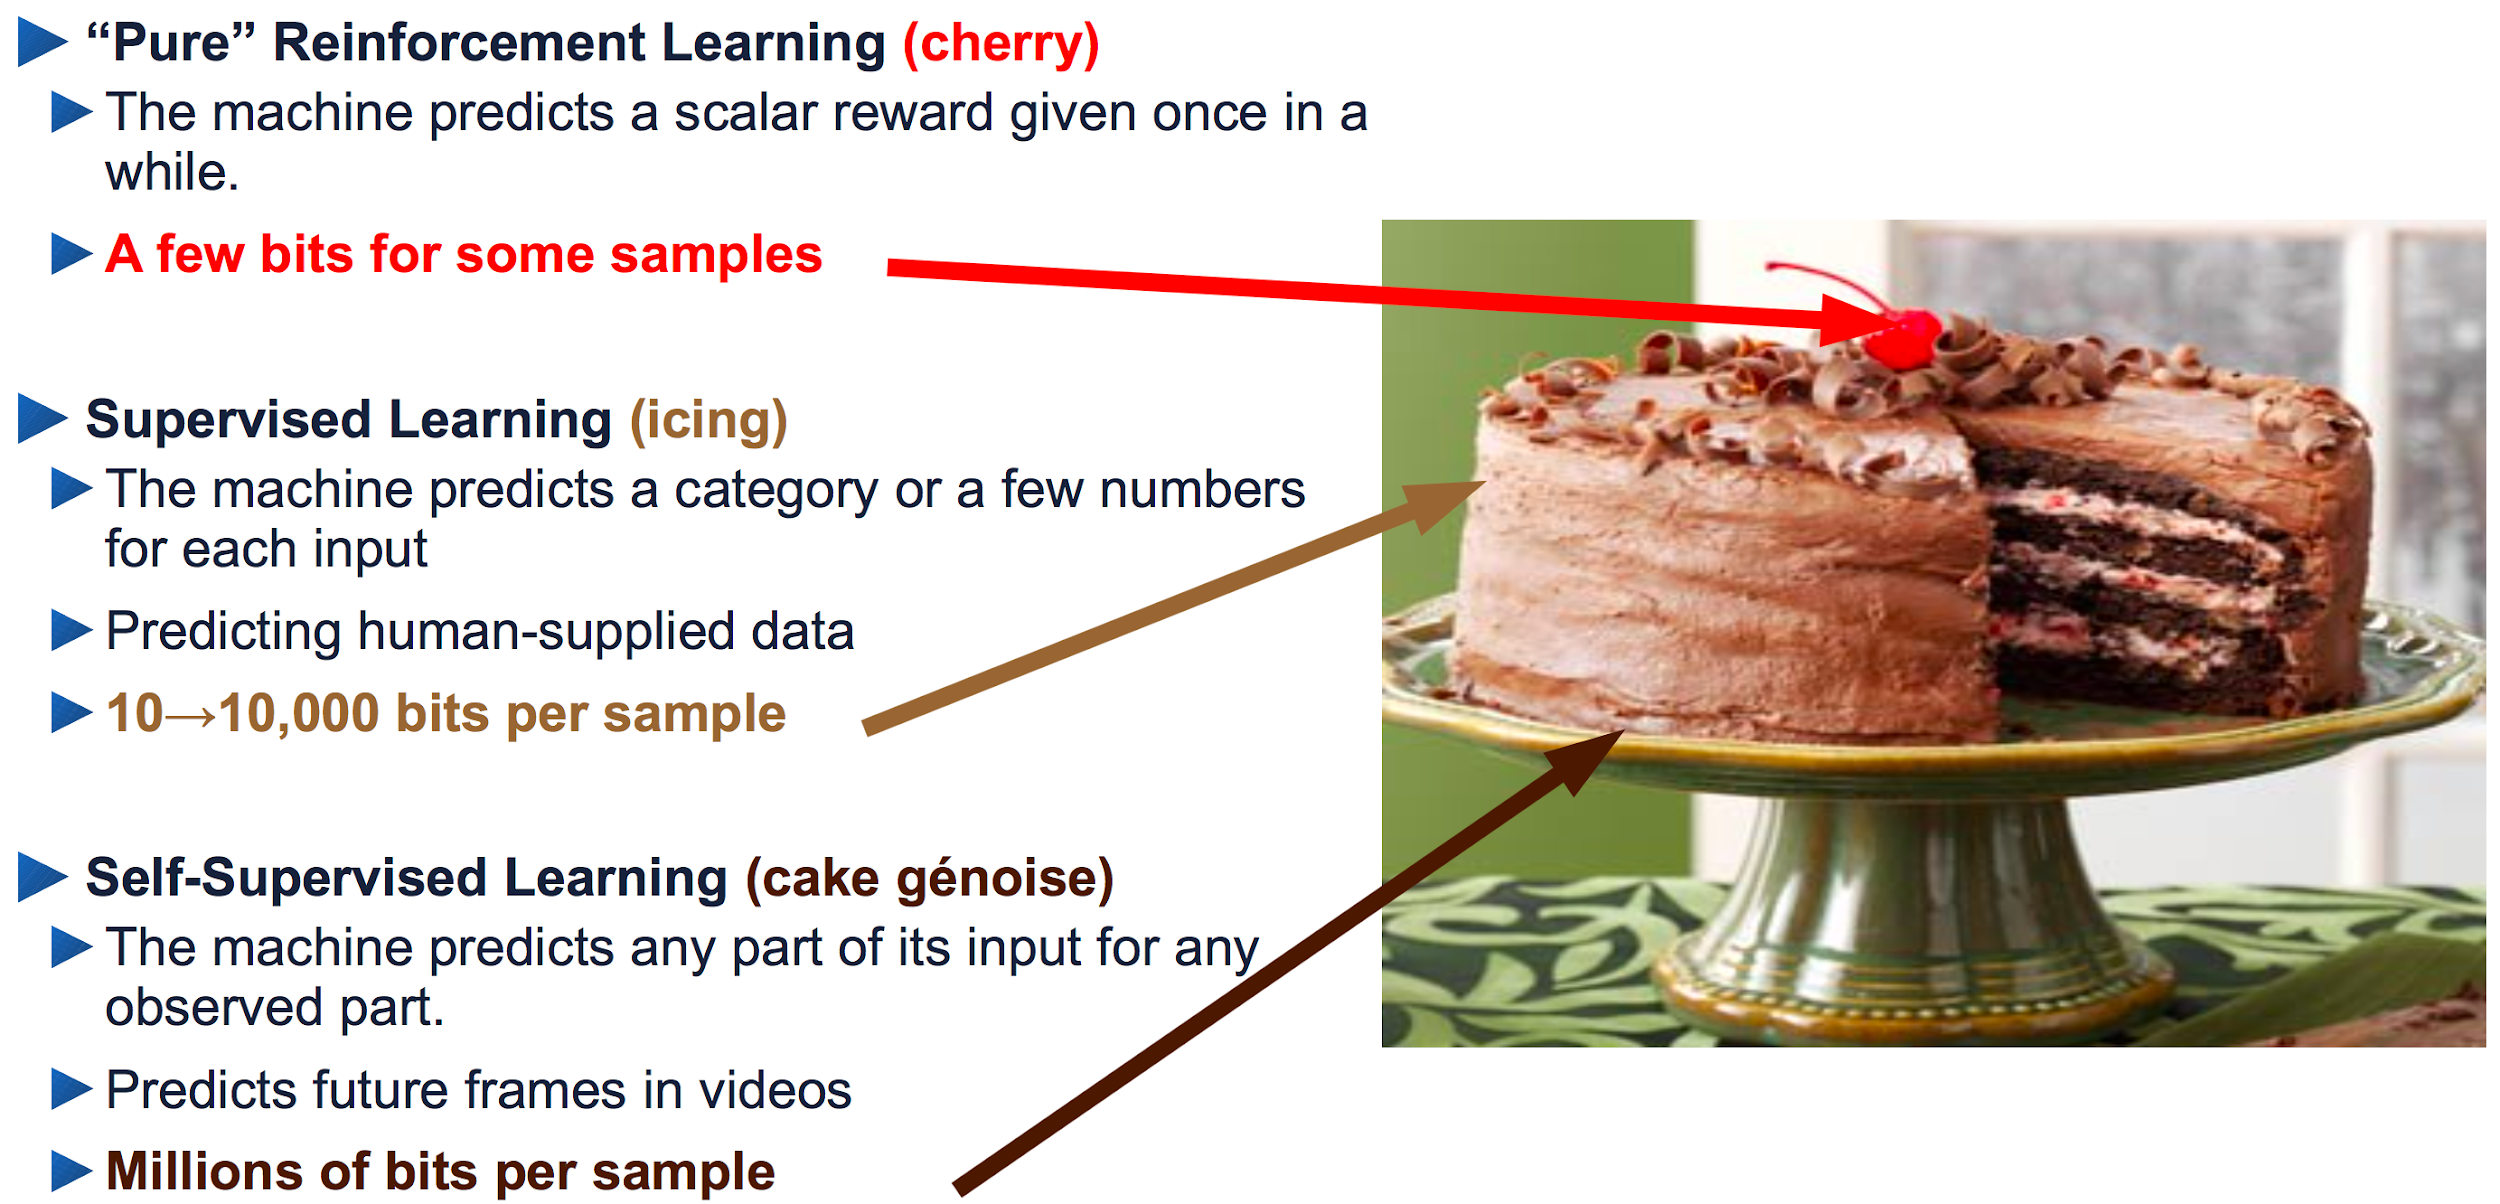
\includegraphics[width=\linewidth,height=\textheight,keepaspectratio]{images/ssl/slide_10_1_img.png}
    \end{figure}

\end{frame}
\begin{frame}[allowframebreaks]{}
    \LARGE Normalizing Flow Models: \\[1.5ex] \textbf{Change of Variables Theorem}
\end{frame}

\begin{frame}[allowframebreaks]{Change of Variables Theorem}
The change of variables formula describe how to evaluate densities of a random variable that is a deterministic transformation from another variable.
\begin{figure}
    \centering
        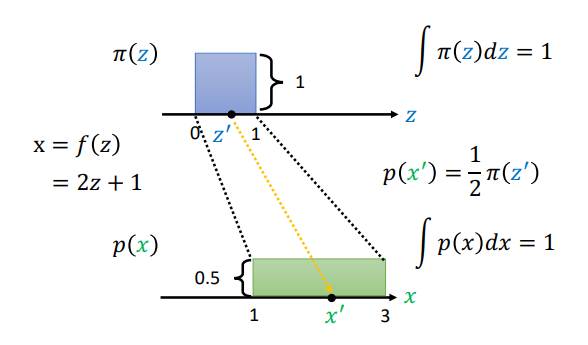
\includegraphics[height=0.6\textheight, width=\textwidth, keepaspectratio]{images/norm-flow/change_var.png}
        \caption*{Transformation of a 1-D random variable to another random variable. Note that the areas of the blue and green rectangles are equal.}
\end{figure}

\framebreak
\begin{figure}
    \centering
    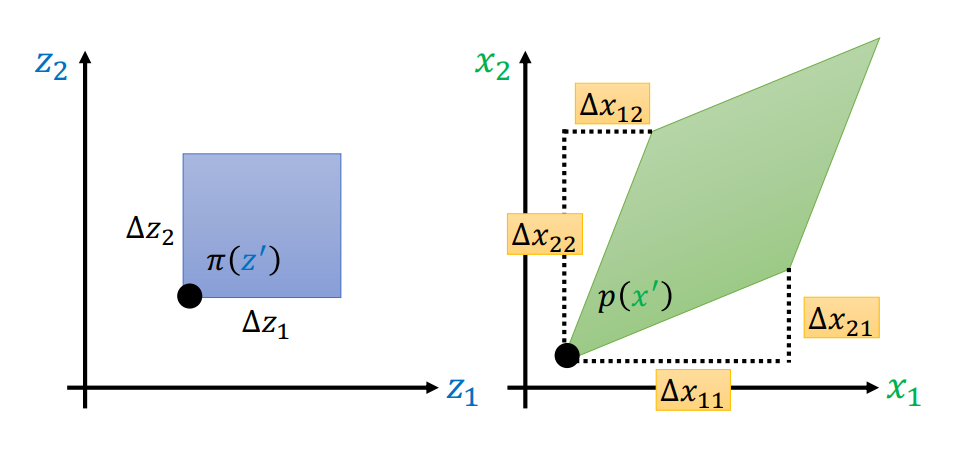
\includegraphics[height=0.7\textheight, width=\textwidth, keepaspectratio]{images/norm-flow/change_var_2.png}
    \caption*{Transformation of a 2-D random variable to another random variable. Note that the areas of the blue and green rectangles are equal.}
\end{figure}

\framebreak

\textbf{Theorem}: Let $Z$ and $X$ be random variables related by a mapping $f:\mathbb{R}^n \rightarrow \mathbb{R}^n$ such that $X = f(Z)$ and $Z = f^{-1}(X)$. Then,
\[
p_X(x) = p_Z(f^{-1}(x)) \left| \det \left( \frac{\partial f^{-1}(x)}{\partial x} \right) \right|
\]
Some important points to note:
\begin{itemize}
    \item $x$ and $z$ must be continuous random variables of the same dimension.
    \item $\frac{\partial f^{-1}(x)}{\partial x}$ is the $n \times n$ \textbf{Jacobian matrix}, where the entry at position $(i, j)$ is $\frac{\partial [f^{-1}(x)]_i}{\partial x_j}$.
    \item For any invertible matrix $A$, $\det(A^{-1}) = [\det(A)]^{-1}$. Therefore, for $z = f^{-1}(x)$,
    \[
    p_X(x) = p_Z(z) \left| \det \left( \frac{\partial f(z)}{\partial z} \right) \right|^{-1}
    \]
\end{itemize}

\framebreak

\large We need:
\begin{itemize}
    \item \textbf{Invertibility of $f$}: The function $f$ must be invertible so that for every $x$ there exists a unique $z = f^{-1}(x)$.
    \item \textbf{Jacobian of $f$}: The Jacobian matrix $\frac{\partial f(z)}{\partial z}$ must be computable and its determinant non-zero almost everywhere to ensure the change of variables formula is valid.
\end{itemize}

\end{frame}
\begin{frame}[allowframebreaks]{}
    \LARGE Normalizing Flow Models: \\[1.5ex] \textbf{Jacobian (2D Case)}
\end{frame}

\begin{frame}[allowframebreaks]{Jacobian (2D Case)}
\begin{itemize}
    \item The Jacobian is a matrix of partial derivatives:
    \[
    J_{ij} = \frac{\partial f_i}{\partial z_j}
    \]
    \item It describes how each component of $f(z)$ changes with $z$.
    \item The Jacobian is needed to compute how volumes change after transformation.
\end{itemize}

\framebreak

\begin{figure}
    \centering
    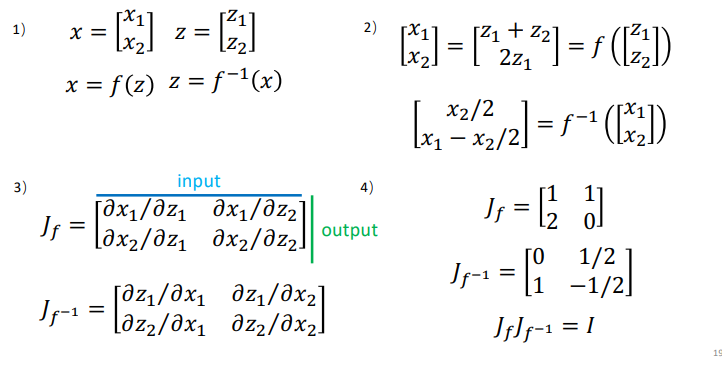
\includegraphics[height=0.8\textheight, width=\textwidth, keepaspectratio]{images/norm-flow/jacobian.png}
    \caption*{Example of a 2D Jacobian matrix. See Appendix~\ref{sec:appendix-jacobian-2d} for more information.}
\end{figure}
    
\end{frame}
\begin{frame}{Matrix Determinant}
The determinant of a \textbf{square matrix} is a \textbf{scalar} that provides information about the matrix.
\begin{figure}
    \centering
    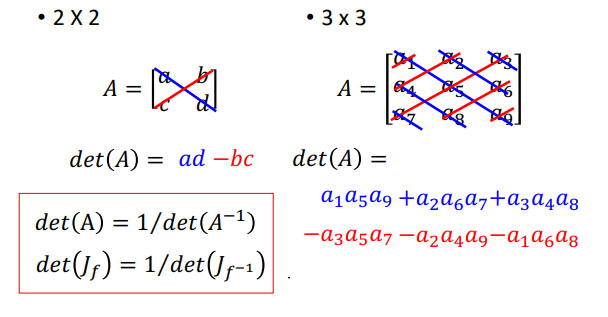
\includegraphics[height=0.8\textheight, width=\textwidth, keepaspectratio]{images/norm-flow/determinant.png}
    \caption*{Example of matrix determinant.}
\end{figure}
    
\end{frame}
\begin{frame}{Generators}
    
\begin{itemize}
    \item A generator $G$ is a network that maps a simple distribution (for example, a normal distribution) $\pi(z)$ to a complex data distribution $p_G(x)$, which aims to be as close as possible to the real data distribution $p_{\text{data}}(x)$.
\end{itemize}
\begin{figure}
    \centering
    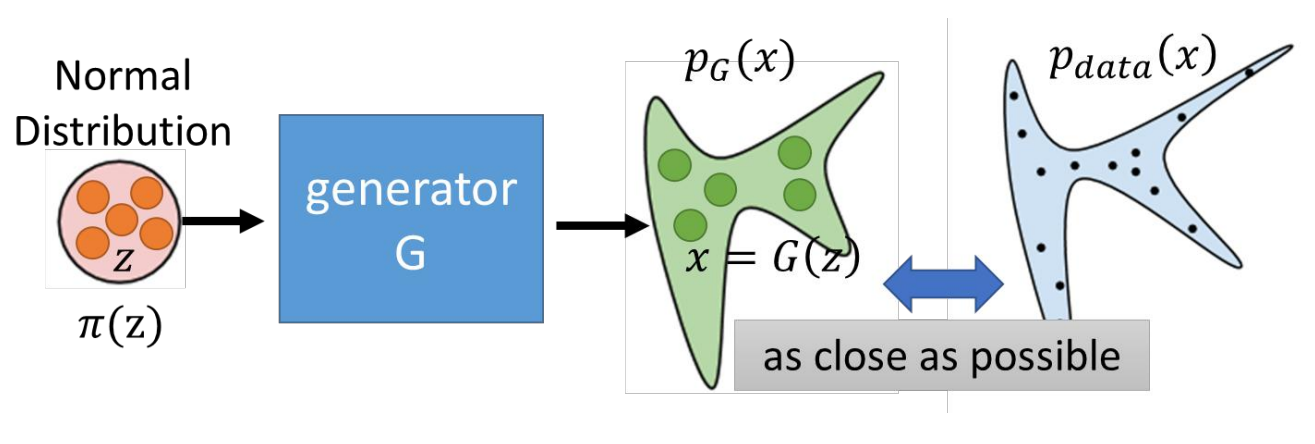
\includegraphics[height=0.5\textheight, width=\textwidth, keepaspectratio]{images/norm-flow/nfm_gen.png}
    \caption*{The goal of a generator network in a generative model}
\end{figure}
\end{frame}

\begin{frame}[allowframebreaks]{Normalizing Flow Models}
    \begin{itemize}
        \item Consider a directed latent-variable model with observed variables $X$ and latent variables $Z$. In a normalizing flow model, the mapping between $Z$ and $X$ is deterministic and invertible: $G:\mathbb{R}^n \rightarrow \mathbb{R}^n$, such that $X=G(Z)$ and $Z=G^{-1}(X)$.
        \item By the change of variables formula, the marginal likelihood $p(x)$ is:
        $$
        p_X(x;\theta) = p_Z(G_\theta^{-1}(x)) \left| \det \left( \frac{\partial G_\theta^{-1}(x)}{\partial x} \right) \right|
        $$
    \end{itemize}
\framebreak

\begin{figure}
    \centering
    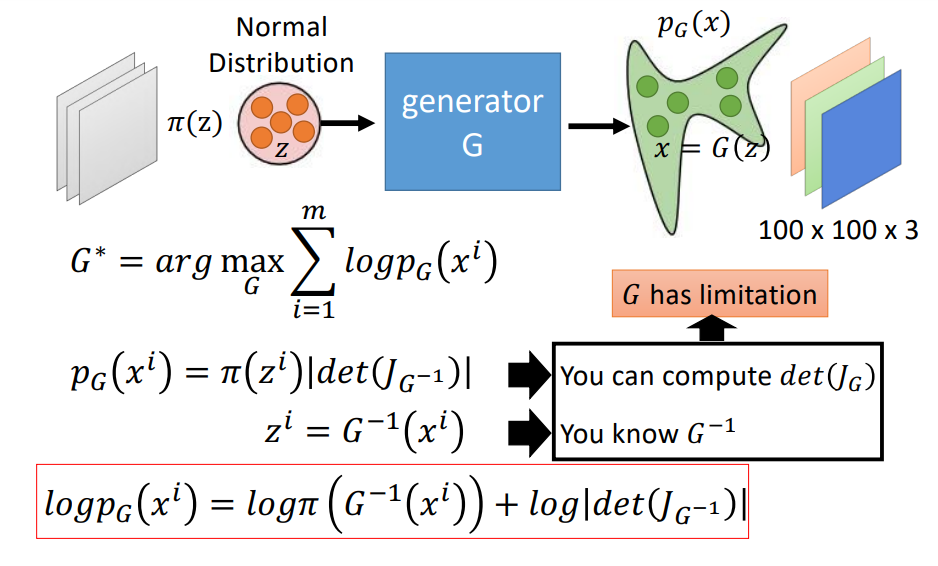
\includegraphics[height=0.9\textheight, width=\textwidth, keepaspectratio]{images/norm-flow/nfm_2.png}
\end{figure}

\framebreak

\begin{itemize}
    \item The expressiveness of $G$ is limited. To model more complex distributions, we need more expressive generators.
\end{itemize}

\begin{figure}
    \centering
    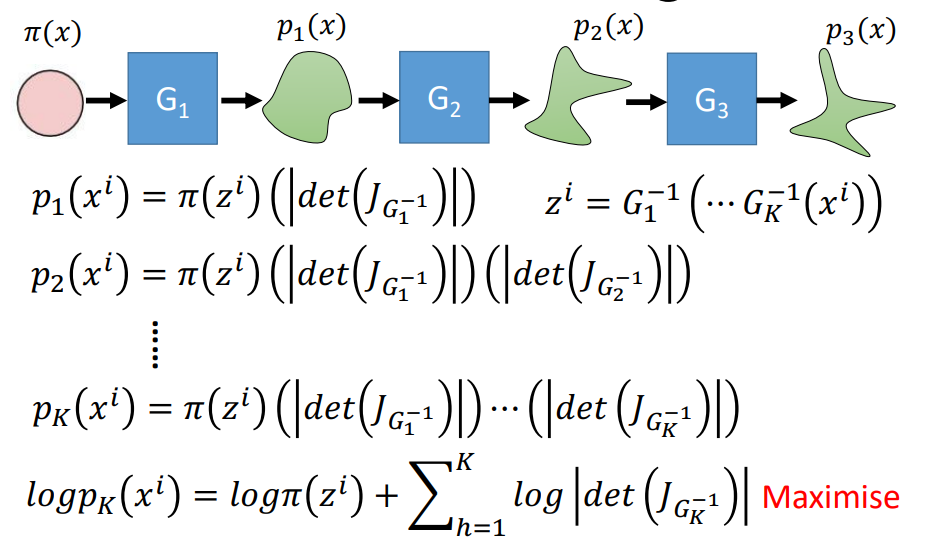
\includegraphics[height=0.9\textheight, width=\textwidth, keepaspectratio]{images/norm-flow/nfm_3.png}
\end{figure}

\framebreak

\begin{itemize}
    \item In practice, we train $G^{-1}$, but use $G$ for generation.
\end{itemize}

\begin{figure}
    \centering
    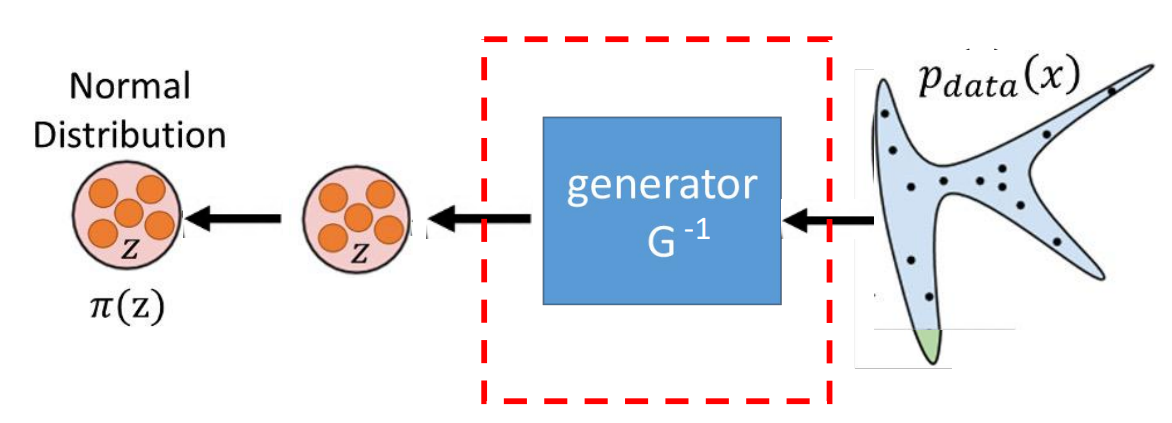
\includegraphics[height=0.5\textheight, width=\textwidth, keepaspectratio]{images/norm-flow/nfm_1.png}
\end{figure}

\framebreak

\begin{itemize}
    \item \textbf{Normalizing}: The change of variables produces a normalized density after applying an invertible transformation.
    \item \textbf{Flow}: Invertible transformations can be composed to create more complex, expressive mappings.
\end{itemize}
\end{frame}
\begin{frame}[allowframebreaks]{}
    \LARGE Normalizing Flow Models: \\[1.5ex] \textbf{Learning and Inference}
\end{frame}

\begin{frame}{Learning and Inference}
\begin{itemize}
    \item Learning is performed via maximum likelihood estimation over the dataset $D$:
    $$
    \max_\theta \log p(D;\theta) = \sum_{x \in D} \left[ \log \pi(G_\theta^{-1}(x)) + \log \left| \det \left( \frac{\partial G_\theta^{-1}(x)}{\partial x} \right) \right| \right]
    $$
    \item Exact likelihood evaluation is achieved using the inverse transformation and the change of variables formula.
    \item Sampling is performed via the forward transformation $G_\theta : Z \rightarrow X$:
    $$
    z \sim \pi(z), \quad x = G_\theta(z)
    $$
    \item Latent representations are inferred via the inverse transformation (no inference network required):
    $$
    z = G_\theta^{-1}(x)
    $$
\end{itemize}
\end{frame}
\begin{frame}[allowframebreaks]{}
    \LARGE Normalizing Flow Models: \\[1.5ex] \textbf{Requirements}
\end{frame}

\begin{frame}[allowframebreaks]{Requirements for Flow Models}
\begin{itemize}
    \item A simple prior $\pi(z)$ that allows for efficient sampling and tractable likelihood evaluation (e.g., Gaussian).
    \item Invertible transformations.
    \item Computing likelihoods also requires evaluating the determinants of $n \times n$ Jacobian matrices, where $n$ is the data dimensionality.
    \begin{itemize}
        \item Computing the determinant of an $n \times n$ matrix is $O(n^3)$, which is prohibitively expensive within a learning loop.
        \item Key idea: Choose transformations so that the resulting Jacobian matrix has a special structure. For example, the determinant of a triangular matrix is the product of its diagonal entries, making it an $O(n)$ operation.
    \end{itemize}
\end{itemize}
\framebreak

\begin{itemize}
    \item We need a fast and simple prior (e.g., Gaussian).
    \item The big question: How do we obtain invertible transformations and efficiently compute the determinants of Jacobians?
    \item \textbf{One solution}: Use coupling layers to design invertible functions and efficiently calculate the determinant of the Jacobian!
\end{itemize}
\end{frame}
\begin{frame}[allowframebreaks]{}
    \LARGE Normalizing Flow Models: \\[1.5ex] \textbf{Coupling layers}
\end{frame}

\begin{frame}[allowframebreaks]{Coupling layers}
\textbf{Concept:}

\begin{itemize}
    \item Split the input $\mathbf{x}$ into two parts: $\mathbf{x} = [\mathbf{x}_1, \mathbf{x}_2]$.
    \item Apply a transformation to one part conditioned on the other:
    \begin{align*}
        \mathbf{y}_1 &= \mathbf{x}_1 \\
        \mathbf{y}_2 &= \mathbf{x}_2 \odot \exp\big(s(\mathbf{x}_1)\big) + t(\mathbf{x}_1)
    \end{align*}
    where $s$ and $t$ are scale and translation functions, respectively.
\end{itemize}

\textbf{Advantages:}
\begin{itemize}
    \item Invertibility is straightforward.
    \item The Jacobian is triangular, making determinant computation efficient.
    \item Facilitates the design of complex, yet tractable, transformations.
\end{itemize}
\begin{figure}
    \centering
    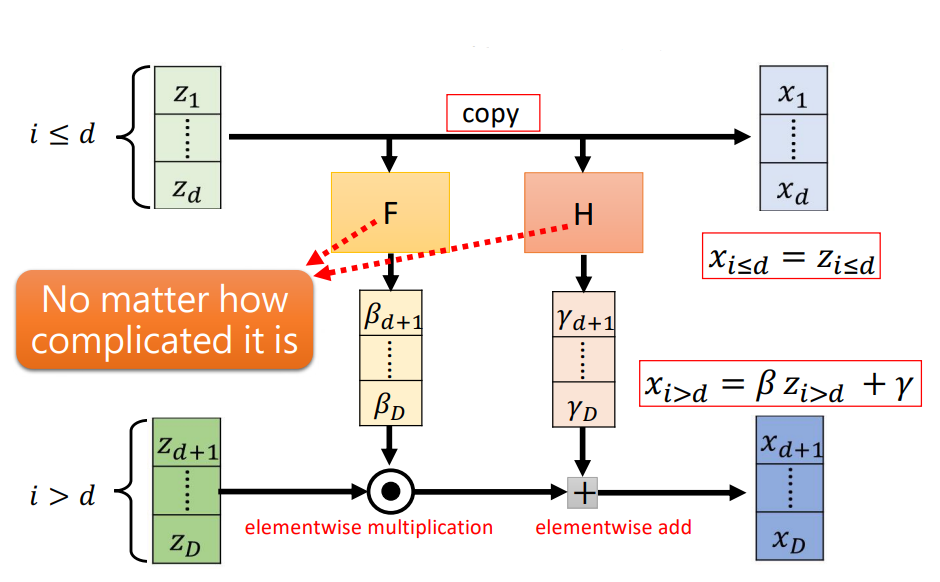
\includegraphics[height=0.9\textheight, width=\textwidth, keepaspectratio]{images/norm-flow/coupling_layer_1.png}
\end{figure}

\framebreak

\begin{figure}
    \centering
    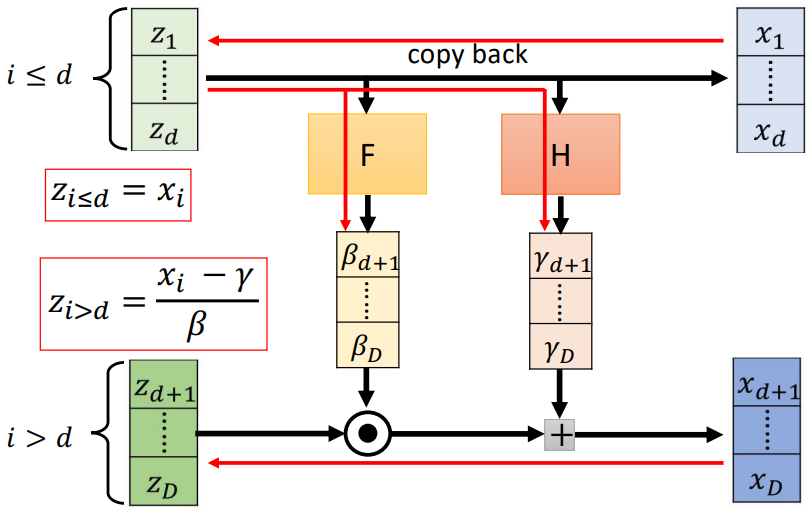
\includegraphics[height=0.9\textheight, width=\textwidth, keepaspectratio]{images/norm-flow/coupling_layer_2.png}
\end{figure}

\framebreak

\begin{figure}
    \centering
    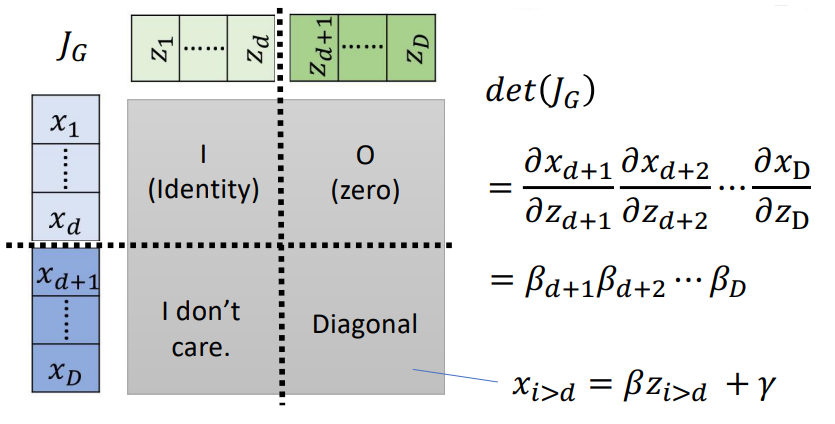
\includegraphics[height=0.9\textheight, width=\textwidth, keepaspectratio]{images/norm-flow/coupling_layer_3.png}
\end{figure}

\framebreak

\begin{figure}
    \centering
    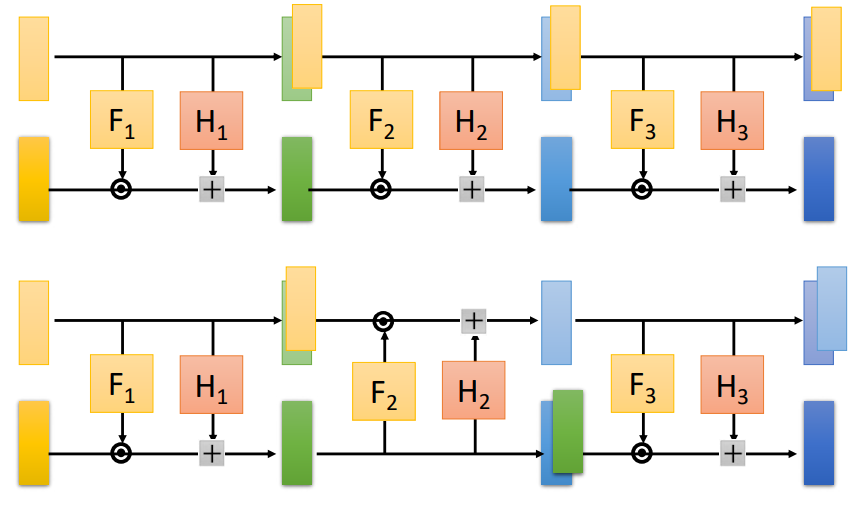
\includegraphics[height=0.9\textheight, width=\textwidth, keepaspectratio]{images/norm-flow/coupling_layer_4.png}
\end{figure}
    
\end{frame}
\begin{frame}[allowframebreaks]{}
    \LARGE Normalizing Flow Models: \\[1.5ex] \textbf{NICE: Nonlinear Independent Components Estimation}
\end{frame}

\begin{frame}[allowframebreaks]{NICE}
\begin{itemize}
    \item \textbf{Overview:} Introduced by Dinh et al. (2014), NICE employs additive coupling layers for constructing invertible transformations.
    \item \textbf{Additive Coupling Layers:}
    \begin{itemize}
        \begin{itemize}
            \item Partition the variables $z$ into two disjoint subsets:
            \item $x_{1:d} = z_{1:d}$
            \item $x_{d+1:n} = z_{d+1:n} + H(z_{1:d})$,
            where $H$ is a neural network.
            \begin{figure}
                    \centering
                    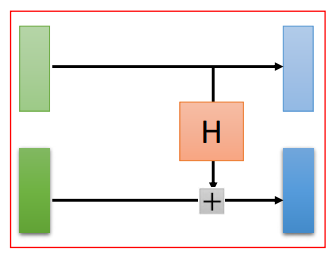
\includegraphics[height=0.4\textheight, width=\textwidth, keepaspectratio]{images/norm-flow/nfm_nice.png}
            \end{figure}
        \end{itemize}
        \item The Jacobian determinant of this transformation is 1, which simplifies density computation.
    \end{itemize}
    \framebreak
    \item Multiple additive coupling layers are composed together, with different partitions in each layer.
    \item \textbf{Limitation:} The transformation is volume-preserving and cannot model changes in volume, which limits expressiveness.
    \item \textbf{Enhancement:} A final rescaling layer is applied to introduce volume changes:
    \begin{align*}
        x = s \odot z
    \end{align*}
    where $s$ is a scaling factor.
\end{itemize}
\end{frame}

\begin{frame}[allowframebreaks]{NICE - Results}
\begin{figure}
    \centering
    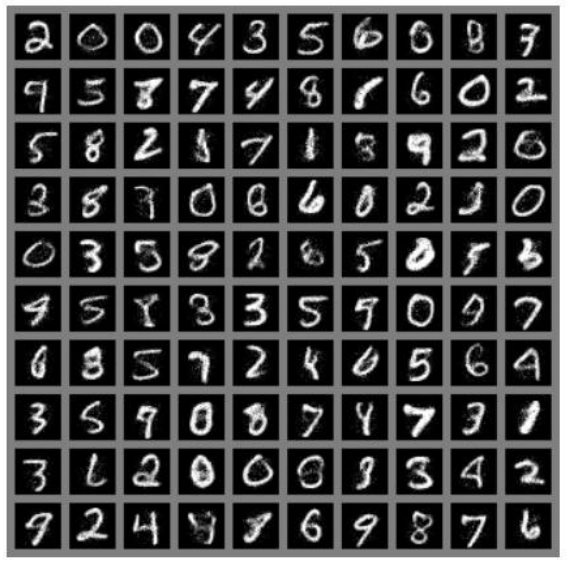
\includegraphics[height=0.8\textheight, width=\textwidth, keepaspectratio]{images/norm-flow/nfm_nice_mnist.png}
    \caption*{NICE generated samples when trained on the MNIST digits dataset.}
\end{figure}

\framebreak

\begin{figure}
    \centering
    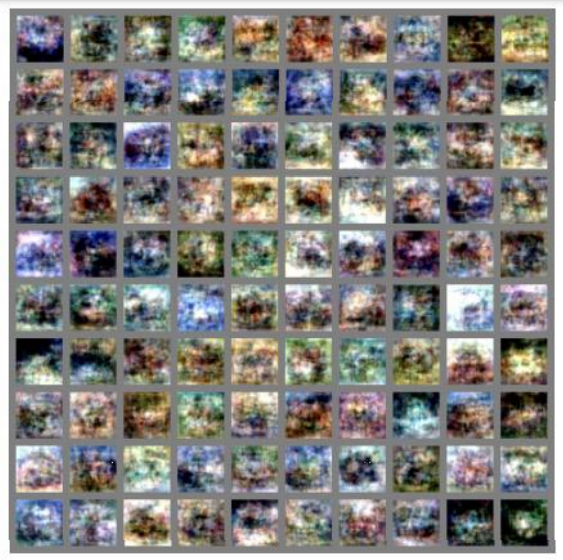
\includegraphics[height=0.8\textheight, width=\textwidth, keepaspectratio]{images/norm-flow/nfm_nice_cifar.png}
    \caption*{NICE generated samples when trained on the CIFAR-10 dataset.}
\end{figure}
    
\end{frame}
\begin{frame}[allowframebreaks]{}
    \LARGE Normalizing Flow Models: \\[1.5ex] \textbf{\Large Real NVP - Real-valued Non-Volume Preserving}
\end{frame}

\begin{frame}[allowframebreaks]{Real NVP}
\textbf{RealNVP: Real-valued Non-Volume Preserving}
\begin{itemize}
    \item Enhancements over NICE:
    \begin{itemize}
        \item Introduces scaling in coupling layers:
        \begin{itemize}
            \item Partition the variables $z$ into two disjoint subsets.
            \item $x_{1:d} = z_{1:d}$
            \item $x_{d+1:n} = z_{d+1:n} \bigodot \exp\left(F(z_{1:d})\right) + H(z_{1:d})$, where $F$ and $H$ are neural networks.
        \end{itemize}
        \begin{figure}
            \centering
            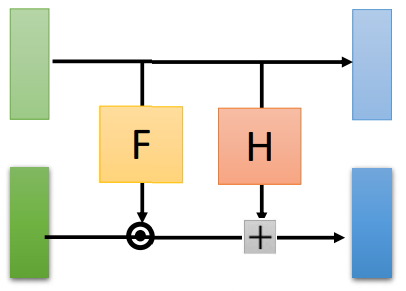
\includegraphics[height=0.4\textheight, width=\textwidth, keepaspectratio]{images/norm-flow/nfm_realnvp.png}
        \end{figure}
        \item Allows modeling of volume changes, increasing flexibility.
    \end{itemize}
    \framebreak
    \item \textbf{Benefits:}
    \begin{itemize}
        \item Efficient computation of the Jacobian determinant due to the triangular structure.
        \item Supports exact likelihood estimation and sampling.
    \end{itemize}
    \item \textbf{Implementation Details:}
    \begin{itemize}
        \item Alternating the roles of $z_{1:d}$ and $z_{d+1:n}$ across layers ensures all dimensions are transformed.
    \end{itemize}
    \item Coupling layers are composed together (with arbitrary partitions of variables in each layer).
    
\end{itemize}
\end{frame}

\begin{frame}{Real NVP - Results}
\begin{figure}
    \centering
    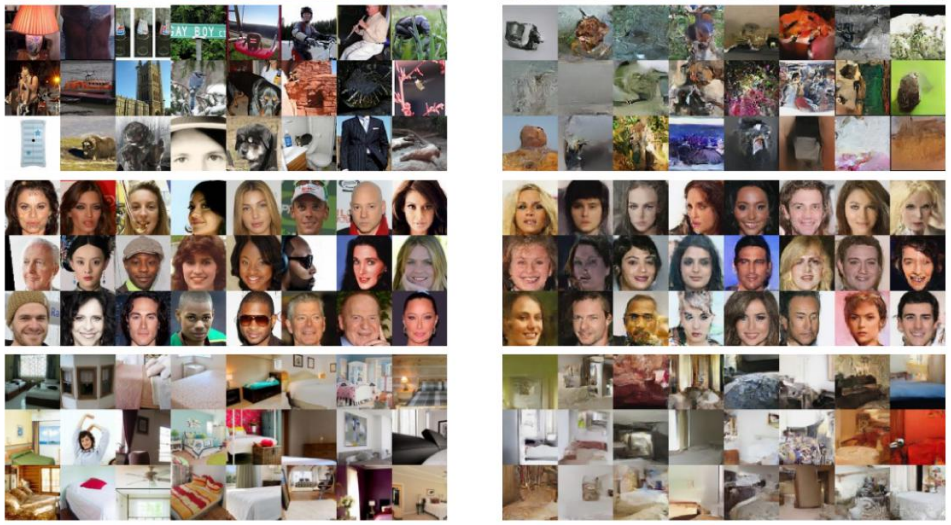
\includegraphics[height=0.8\textheight, width=\textwidth, keepaspectratio]{images/norm-flow/nfm_realnvp_results.png}
    \caption*{Real NVP generated samples}
\end{figure}
\end{frame}
\begin{frame}[allowframebreaks]{}
    \LARGE Normalizing Flow Models: \\[1.5ex] \textbf{Glow: Generative Flow}
\end{frame}

\begin{frame}[allowframebreaks]{Glow}
\textbf{Innovations:}

Introduced by Kingma and Dhariwal (2018), Glow incorporates:
\begin{itemize}
    \item \textbf{Invertible $1\times1$ convolutions} for channel mixing.
    \item \textbf{ActNorm layers} for data-dependent normalization.
    \item \textbf{Affine coupling layers} similar to RealNVP.
\end{itemize}

\textbf{Advantages:}
\begin{itemize}
    \item Improved expressiveness and stability.
    \item Enhanced performance in image generation tasks.
\end{itemize}
\framebreak
\textbf{Key Components:}
\begin{itemize}
    \item \textbf{ActNorm:} Applies per-channel affine transformation initialized with data statistics.
    \item \textbf{Invertible $1\times1$ Convolution:} Generalizes permutation operations, allowing learned channel mixing.
    \item \textbf{Affine Coupling Layers:} As in RealNVP, but integrated with the above components for greater flexibility.
\end{itemize}

\begin{figure}
    \centering
    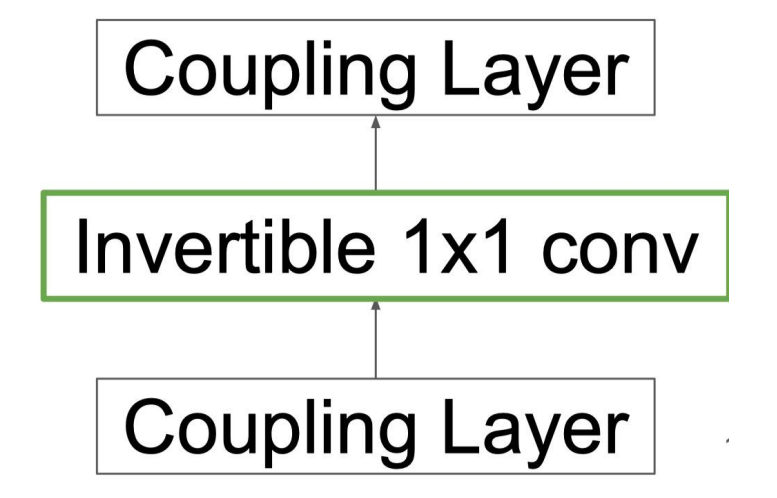
\includegraphics[height=0.4\textheight, width=\textwidth, keepaspectratio]{images/norm-flow/nfm_glow.png}
\end{figure}

\framebreak

\begin{figure}
    \centering
    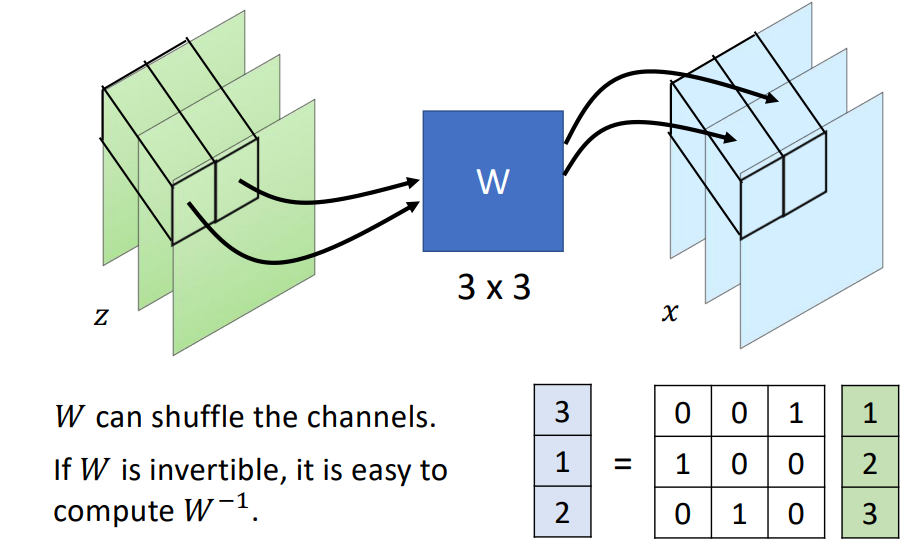
\includegraphics[height=0.9\textheight, width=\textwidth, keepaspectratio]{images/norm-flow/nfm_glow_1.png}
\end{figure}
\end{frame}

\begin{frame}[allowframebreaks]{Glow - Results}
\begin{figure}
    \centering
    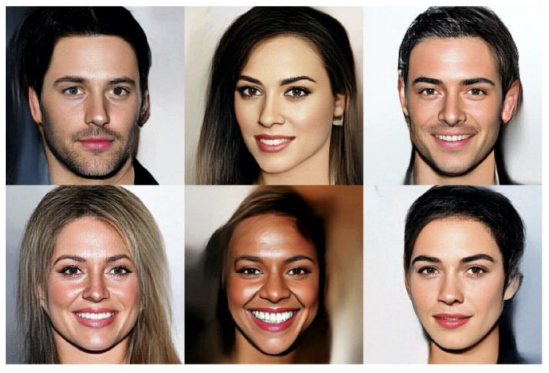
\includegraphics[height=0.8\textheight, width=\textwidth, keepaspectratio]{images/norm-flow/nfm_glow_results_1.png}
    \caption*{Glow generated samples}
\end{figure}

\framebreak

\begin{figure}
    \centering
    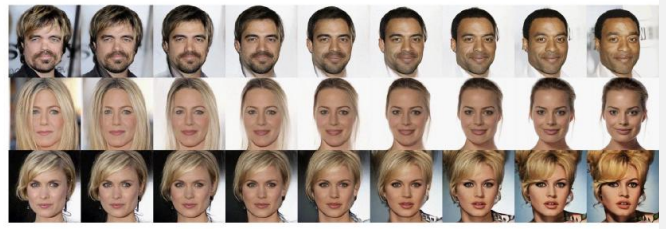
\includegraphics[height=0.8\textheight, width=\textwidth, keepaspectratio]{images/norm-flow/nfm_glow_results_2.png}
    \caption*{Linear interpolation in latent space between real images with Glow}
\end{figure}
\end{frame}
\begin{frame}[allowframebreaks]{Summary}
\begin{itemize}
    \item \textbf{SimCLR:}
    \begin{itemize}
        \item Simple framework for contrastive learning.
        \item Uses data augmentation and contrastive loss.
    \end{itemize}
    \item \textbf{BYOL:}
    \begin{itemize}
        \item Self-supervised approach without negative pairs.
        \item Uses two networks: online and target.
    \end{itemize}
    \item \textbf{DINO:}
    \begin{itemize}
        \item Self-distillation method without labels.
        \item Uses teacher-student networks and knowledge distillation.
    \end{itemize}

    \framebreak

    \item \textbf{DINOv2:}
    \begin{itemize}
        \item Improved version of DINO.
        \item Enhanced training strategies and architectures.
        \item Better performance and scalability.
    \end{itemize}
    \item \textbf{iBOT:}
    \begin{itemize}
        \item Combines contrastive learning with masked image modeling.
        \item Uses BERT-style pretraining and vision transformers.
    \end{itemize}
\end{itemize}
\end{frame}
\begin{frame}{}
    \LARGE Advanced Diffusion Models: \textbf{Limitations}
\end{frame}

\begin{frame}{Limitations}
\begin{tabular}{p{3.5cm} p{8cm}}
\textbf{Challenge} & \textbf{Explanation} \\
\hline
Compute cost & Denoising many steps can be slow / costly \\[0.8em]
Biases \& ethics & Models reflect biased training data \\[0.8em]
Guide artifacts & High guidance can oversharpen or distort \\[0.8em]
Fine-tune data needs & Requires quality, diverse data \\[0.8em]
Legal concerns & Generated content may face IP issues \\
\end{tabular}
\end{frame}
\section{References \& Resources}
\begin{frame}{}
    \LARGE CNN: \textbf{References \& Resources}
\end{frame}

\begin{frame}[allowframebreaks]{References \& Resources}
    \begin{thebibliography}{99}
        \bibitem{cs231n}
            Stanford CS231n Lecture Notes.\\
            \url{http://cs231n.stanford.edu/}
        \bibitem{goodfellow}
            Ian Goodfellow, Yoshua Bengio, and Aaron Courville.\\
            \textit{Deep Learning}, Chapter 9.
        \bibitem{pytorch}
            PyTorch Official Documentation.\\
            \url{https://pytorch.org/docs/}
        \bibitem{brownlee}
            Jason Brownlee.\\
            A Guide to CNNs.\\
            \url{https://machinelearningmastery.com/}
        \bibitem{krizhevsky2012}
            Alex Krizhevsky, Ilya Sutskever, and Geoffrey E. Hinton.\\
            "ImageNet Classification with Deep Convolutional Neural Networks."\\
            NIPS 2012.
        \bibitem{distill}
            Visualizing CNNs.\\
            \url{https://distill.pub/2017/feature-visualization/}
    \end{thebibliography}
\end{frame}
\begin{frame}[allowframebreaks]{Appendix}
\begin{block}{GANs: Definition and Core Components:}
    \begin{itemize}
        \item \textbf{Definition}: Generative Adversarial Networks (GANs) consist of two neural networks trained in opposition to each other.
        \item \textbf{Core Components:}
        \begin{itemize}
            \item \textbf{Generator (G):} Takes random noise (latent vector) and produces fake data samples.
            \item \textbf{Discriminator (D):} Receives real or fake data and predicts whether the input is real.
        \end{itemize}
        \item \textbf{Mathematical Formulation:}
    \end{itemize}
    \begin{equation*}
        \min_G \max_D \; \mathbb{E}_{x \sim p_{\text{data}}} [\log D(x)] + \mathbb{E}_{z \sim p_z} [\log(1 - D(G(z)))]
    \end{equation*}
    \begin{itemize}
        \item[] Where:
        \begin{itemize}
            \item $x$: Real data sample
            \item $z$: Noise vector sampled from prior $p_z$
            \item $G(z)$: Generated sample
        \end{itemize}
    \end{itemize}
\end{block}


\end{frame}


\begin{frame}[plain]
  \frametitle{Credits}
  \begin{center}
    \textbf{Credits} \\[1.5em]

    \Large Dr. Prashant Aparajeya \\[0.5em]
    {\normalsize Computer Vision Scientist | Director(AISimply Ltd)} \\[0.5em]
    \footnotesize \href{mailto:p.aparajeya@aisimply.uk}{p.aparajeya@aisimply.uk} \\[2em]

    {\footnotesize This project benefited from external collaboration, and we acknowledge their contribution with gratitude.}
  \end{center}
\end{frame}


\end{document} 